\chapter{Methodology}
\section{Introduction}
The overall purposes of this study is to improve efficiencies of \gls{ic}'s digital document management strategies. 
The study involves investigating internal \gls{ic}'s working procedures and regulations.
How \gls{ic} execute strategies on their digital document assets.
What are advantages and disadvantages of their strategies.
Gaining such information is valuable to this study because plausible solutions could be proposed and implemented. 
Solutions that could further improve flows of documents inside \gls{ic}.
This chapter presents reasonable research methods to address the research questions.
Conceptual design will also be introduced to provide an abstract model of this experiment.

\section{Gathering Requirements}
Section \ref{sec:motivation} introduced digital document problems occurred inside \gls{ic}.
These problems were formulated to research questions suitable for this study.
The study's goal is to create a system to verify the hypotheses posed by two research questions:
\begin{enumerate}
	\item How to store and retrieve digital \gls{ic}'s documents so that authorized users can access within \gls{ic}, \gls{kmitl} precinct?
	\item How to track \gls{ic}'s document going through each task specified by \gls{ic}'s document workflow?
\end{enumerate}
This study implements qualitative research method with two research strategies: interview and case study.
The following sections discuss these two strategies in more detail.

\subsection{Interview}
\citeauthor{gall7j} (\citeyear{gall7j}) states that interview is the spontaneous generation of questions in a natural interaction, typically one that occurs as part of ongoing participant observation fieldwork.
\citeauthor{brady2011craft} (\citeyear{brady2011craft}) points out that what interviewer and salesman have in common is potential customers whom one could hold their attention to talk.
Getting an interview means making an appointment to see the subject, identifying questions related to the research topic, and showing on time for the interview.
The purpose of interview is to gain information from interviewee by having interviewer asking questions.
Researchers can gain useful insights from the subject who is expertise in one's field.

Figure \ref{ic-org-sturcture} shows \gls{ic}'s organization structure.
The top-most is the dean followed by deputy dean then assistant of deputy dean.
On the right hand side are committee members.
Only academic and academic support located at the bottom-most hierarchy involves archiving documents.
 \begin{figure}[h]
 	\centering
 	\caption{\gls{ic} organization's structure}
 	\label{ic-org-sturcture}
 	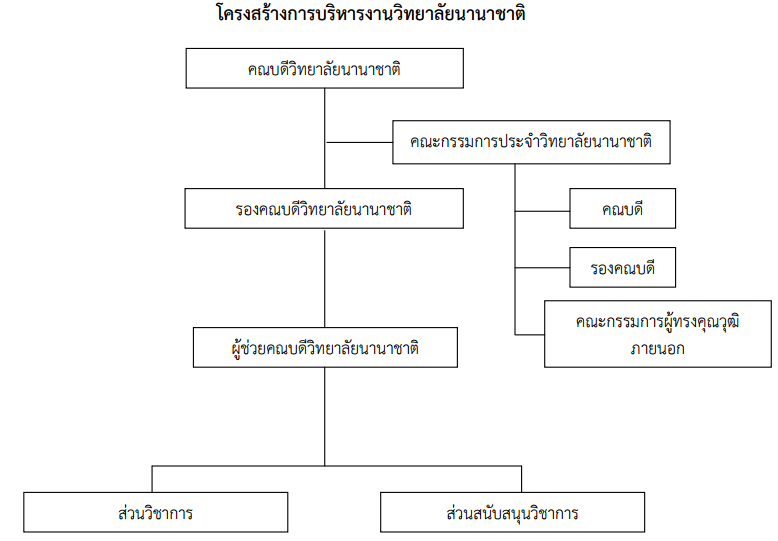
\includegraphics[scale=0.7]{res/Methodology/ic-org}
 \end{figure}

In this study, \gls{ic} staffs are the subject of this study divided into two focus groups:
\begin{description}
	\item [Academic staffs (the buttom-most hierarchy)] as a primary focus group because they are responsible for keeping records of all \gls{ic}'s documents.
	Transfer documents around the organization according to \gls{ic}'s workflow specifications.
	Managing day-to-day operations within the organization.
	They also provide academic advices and guidances to \gls{ic} undergraduate and postgraduate students.

	\item [Administrative staffs] as a secondary focus group because they are not directly involve in keeping and organizing documents.
	Some of them have privilege to issue, review, and approve documents.
	In order to know more about their procedures, deputy dean and deputy dean's assistant are selected as a sample for this study.
\end{description}

After conducted an interview, \gls{ic} staffs reveal that they would like a system that manage their organization's documents automatically.
What they mean by managing is that they would like to know what are they suppose to do with received documents.
Things they have to do could be approval, signing, printing, or commenting on documents.
Then, forwarding the document to another person in the organization without necessarily having to know who that person is.
They also would like to know any additional documents required before forwarding documents so that they can prepare them beforehand.

For every official \gls{ic}'s documents, \gls{ic} assigns an identification number internally after the document got approved by the higher-ups.
There are eleven types of documents separated into three categories based on head of the department who is responsible for those documents as shown in table \ref{tbl-doc-subtype}.
\begin{table}[h]
	\caption{Document type with identification code separated by category}
	\label{tbl-doc-subtype}
	\centering
\begin{tabular}{llC{3cm}}
	\hline
	Category & Document Type & Identification Code \\
	\hline
	General Management 1 & Archive & AA \\
	General Management 1 & Human Resources & AB \\
	General Management 1 & Quality Assurance & AC \\
	General Management 1 & Parcel & AD \\
	General Management 1 & IT/KM & AE \\
	\midrule
	General Management 2 & Plan and Risk Management & BA \\
	General Management 2 & Accounting & BB \\
	General Management 2 & Research & BC \\
	General Management 2 & Academic Management & BD \\
	\midrule
	Academic & Academic Administration & CA \\
	Academic & Student Affairs & CB \\
	\hline
\end{tabular}
\end{table}

According to the scope stated in section \ref{sec:scope}, each documents are associated with the document as shown in table \ref{tbl-scope-doc-subtype}.
External documents are not \gls{ic}'s official documents in table \ref{tbl-doc-subtype}.
They are attachments of the official document.
\begin{table}
	\centering
	\caption{Association between document stated in \ref{sec:scope} and document type in table \ref{tbl-doc-subtype}}
	\label{tbl-scope-doc-subtype}
\begin{tabular}{ll}
	Document Form & Document Type \\
	\hline
	Absence Form & Academic Administration \\
	Student Internship Form & Student Affairs \\
	Conference Outside \gls{kmitl} Form & Academic Administration \\
	\hline
\end{tabular}
\end{table}

\subsection{Case Study}
\citeauthor{merriam1988case} (\citeyear{merriam1988case}) defines case study as an intensive study of a single unit for the purpose of understanding a larger class of similar units.
Unit refers to an observed sample at a discrete point in time.
Each unit comprises of cases built from variables upon observations.
For example, an analysis of worldwide smartphone sales in fourth quarter of 2011 \cite{goasduff2012gartner}.
Samples are mobile devices.
Units are worldwide mobile sales to end users observed in fourth quarter of 2010 and 2011.
Cases are sales by vendor and sales by operating system.
Variables are total number of sales (thousands of units) and market share percentage.
Figure \ref{tbl:ex-case-study-var} shows \citeauthor{goasduff2012gartner}'s case study \cite{goasduff2012gartner} in hierarchy based on \citeauthor{merriam1988case}'s definition.
A unit (sales in fourth quarter) are constructed from two sub units based on years---2010 and 2011.
Sub units in figure \ref{tbl:ex-case-study-var} are split to another column to preserve space.

\begin{figure}[h]
	\caption{Samples, units, cases, and variables for \citeauthor{goasduff2012gartner}'s case study \cite{goasduff2012gartner}}
	\label{tbl:ex-case-study-var}
\begin{tabular}{ll}
	\begin{minipage}{8cm}\dirtree{%
		.1 Mobile Devices.
			.2 Sales in Fourth Quarter.	
				.3 2010.
					.4 By Vendor.
						.5 Total Sales (Thousands of Units).
						.5 Market Share (\%).
					.4 By Operating System.
						.5 Total Sales (Thousands of Units).
						.5 Market Share (\%).
		}
	\end{minipage}
	&
	\begin{minipage}{8cm}\dirtree{%
		.1 Mobile Devices.
			.2 Sales in Fourth Quarter.	
				.3 2011.
					.4 By Vendor.
						.5 Total Sales (Thousands of Units).
						.5 Market Share (\%).
					.4 By Operating System.
						.5 Total Sales (Thousands of Units).
						.5 Market Share (\%).
		}
	\end{minipage}
\end{tabular}
\end{figure}

Conducting case studies based on \citeauthor{merriam1988case}'s definition can yield concrete results.
\citeauthor{merriam1988case}'s definition offers an advantage to study the same case in different point of time.
It also allows variables to be unquantifiable as \citeauthor{merriam1988case} states that variables are built from observation.
This goes along with the qualitative research method that relies on inquiring and investigating to decide a course of action.

This study utilizes \citeauthor{merriam1988case}'s case study model to construct case studies as shown in figure \ref{fig:our-case-study-method}.
Documents are a sample.
\gls{ic}'s documents observed in 2015 is a unit.
There are three cases;
\begin{enumerate*}
	\item storing digital documents;
	\item retrieving digital documents;
	\item tracking digital documents.
\end{enumerate*}
First and second unit comes from the second research question.
Thrid unit comes from the third research question.
Each case comprises of four variables;
\begin{enumerate*}
	\item absence form;
	\item student internship form;
	\item conference outside \gls{kmitl} form;
	\item external document.
\end{enumerate*}
They come from the scope stated in section \ref{sec:scope}.

\begin{figure}[h!]
	\centering
	\caption{Samples, units, cases, and variables for case study of this research}
	\label{fig:our-case-study-method}
	\begin{minipage}{8cm}\dirtree{%
		.1 Documents.
		.2 \gls{ic}'s Documents Observed in 2015.
		.3 Storing Digital Documents.
		.4 Absence Form.
		.4 Student Internship Form.
		.4 Conference Outside \gls{kmitl} Form.
		.4 External Digital Documents.
		.3 Retrieving Digital Documents.
		.4 Absence Form.
		.4 Student Internship Form.
		.4 Conference Outside \gls{kmitl} Form.
		.4 External Digital Documents.
		.3 Tracking Digital Documents.
		.4 Absence Form.
		.4 Student Internship Form.
		.4 Conference Outside \gls{kmitl} Form.
		.4 External Digital Documents.
		}
	\end{minipage}
\end{figure}

